\section{Results}

% most interesting results first and those i was formulating hypotheses about!!
% in this case here its first the contingency table and then the number of steps taken until convergence

Our most important finding was that it did not matter what feedback was fed to the RL agent. The agent's convergence performance was not affected by the feedback origin ($statistic = X, p = Y$). Furthermore, convergence speed was comparable as well ($t_{(11)} = X, p = Y$).

The contingency table in figure~\ref{res:cm_table} shows ...
\begin{figure} % this and res:steps will be one figure with A and B lettering
    \centering
    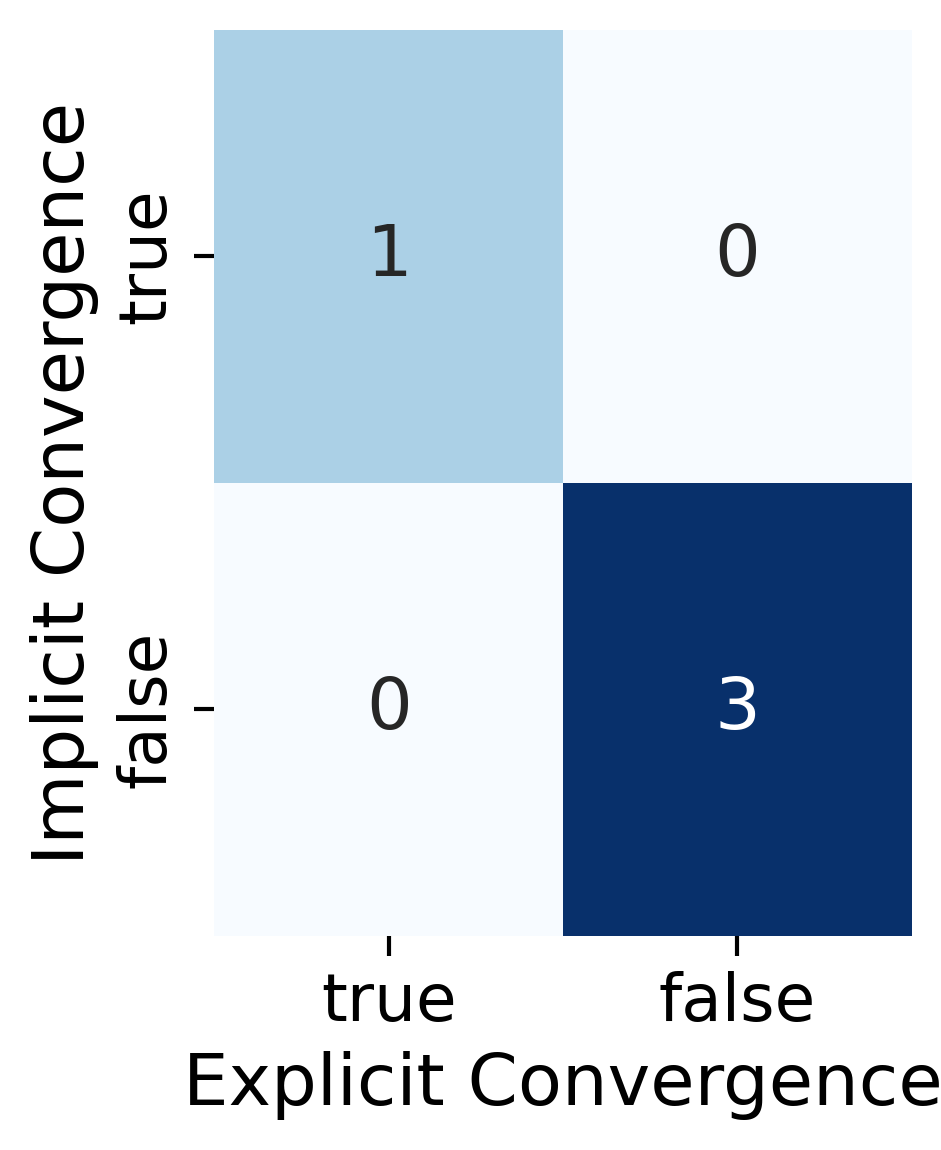
\includegraphics[width=0.5\linewidth]{input/img/impl_explc_contingeny_table.png}
    \caption{Contingency table of implicit and explicit convergence states, with color intensity representing frequency.}
    \Description{A contingency table showing the frequency of implicit and explicit convergence states, with rows for implicit states, columns for explicit states, and color intensity indicating frequency.}
    \label{res:cm_table}
\end{figure}

\begin{figure}
    \centering
    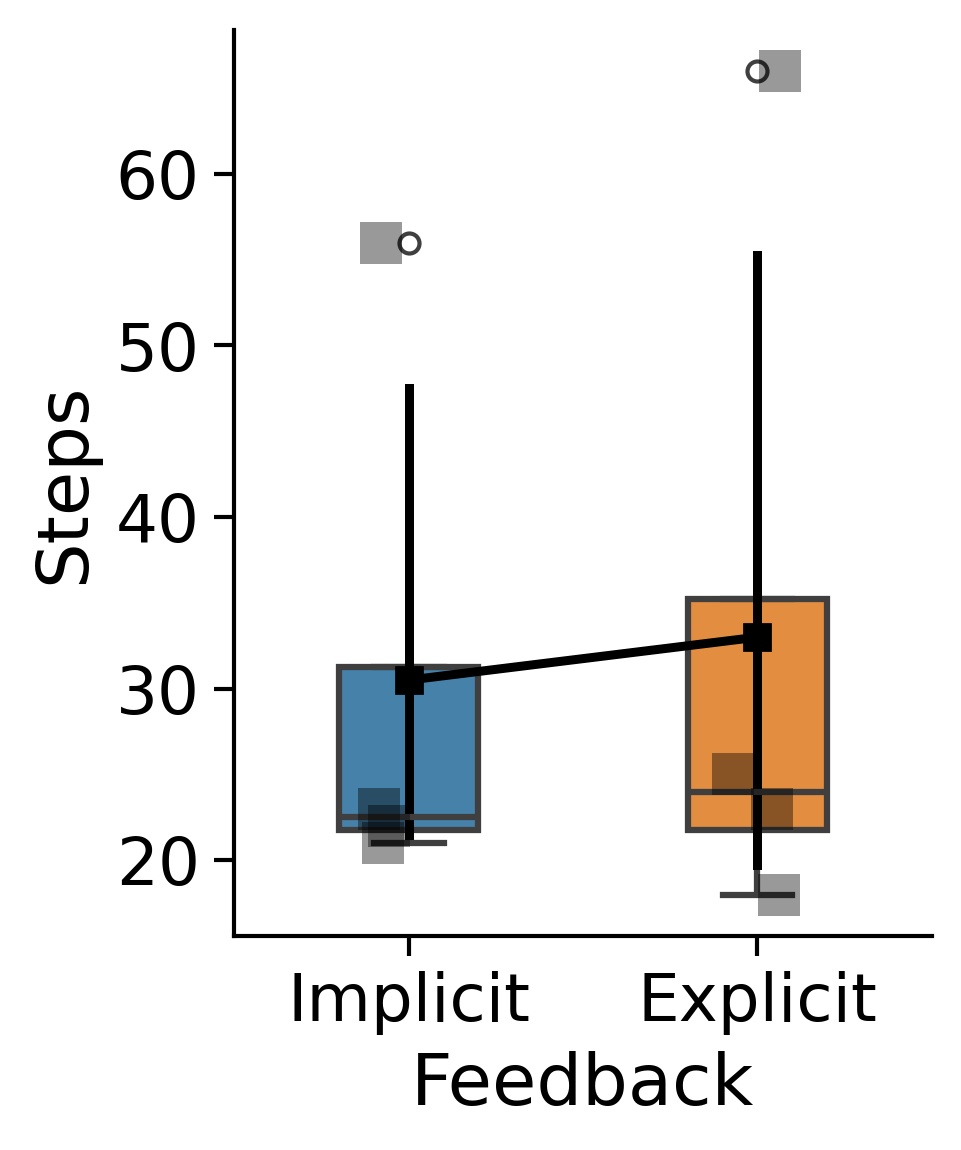
\includegraphics[width=0.5\linewidth]{input/img/impl_explc_steps.png}
    \caption{Box plot of steps until stoppage for implicit and explicit feedback conditions. Medians are shown within each box, with an overlaid line for the mean trend. Black circles indicate outliers, and grey squares represent individual participants.}
    \Description{Box plot of steps until stoppage for implicit and explicit feedback conditions. The central line in each box represents the median, while the overlaid black line indicates the mean trend across conditions. Black circle markers denote outliers. Grey squares denote single participants.}
    \label{res:steps}
\end{figure}



\begin{figure}
    \centering
    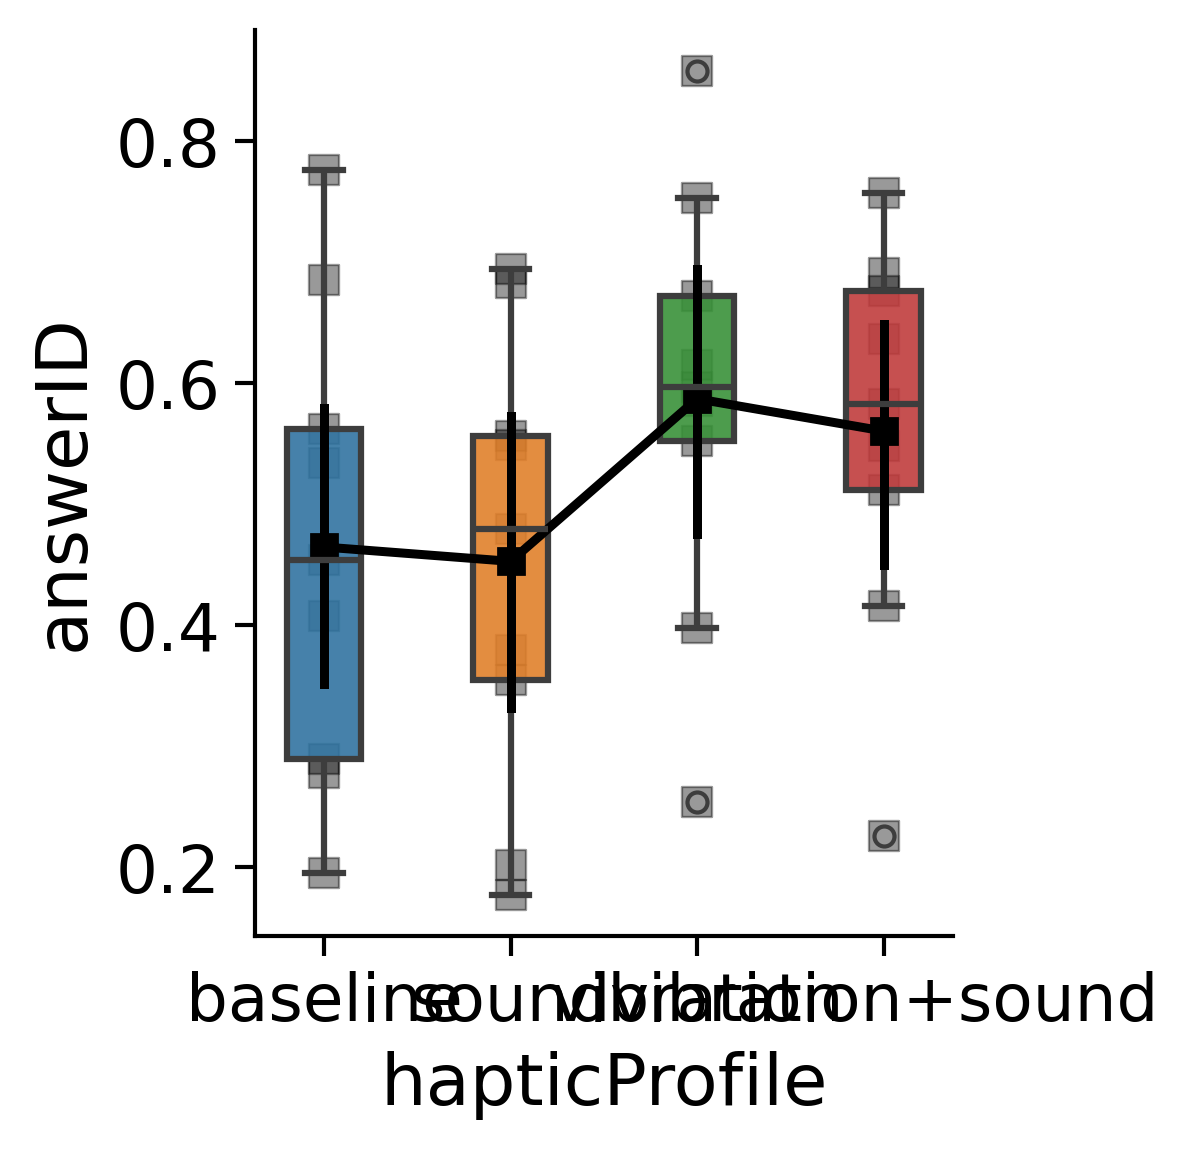
\includegraphics[width=0.5\linewidth]{input/img/answerID.png}
    \caption{Box plot of ratings in the training block across haptic profiles. Medians are shown within each box, with black circles indicating outliers. The overlaid line represents the mean trend, and grey squares denote individual participants.}
    \Description{Box plot of explicit ratings in the training block across different haptic profiles (baseline, sound, vibration, and vibration+sound). The central line in each box represents the median, while the black circle markers indicate outliers. The overlaid line plot shows the mean trend across conditions. Grey squares denote single participants.}
    \label{res:answerID}
\end{figure}

% now EEG findings
\begin{figure*}[!ht]
    \centering
    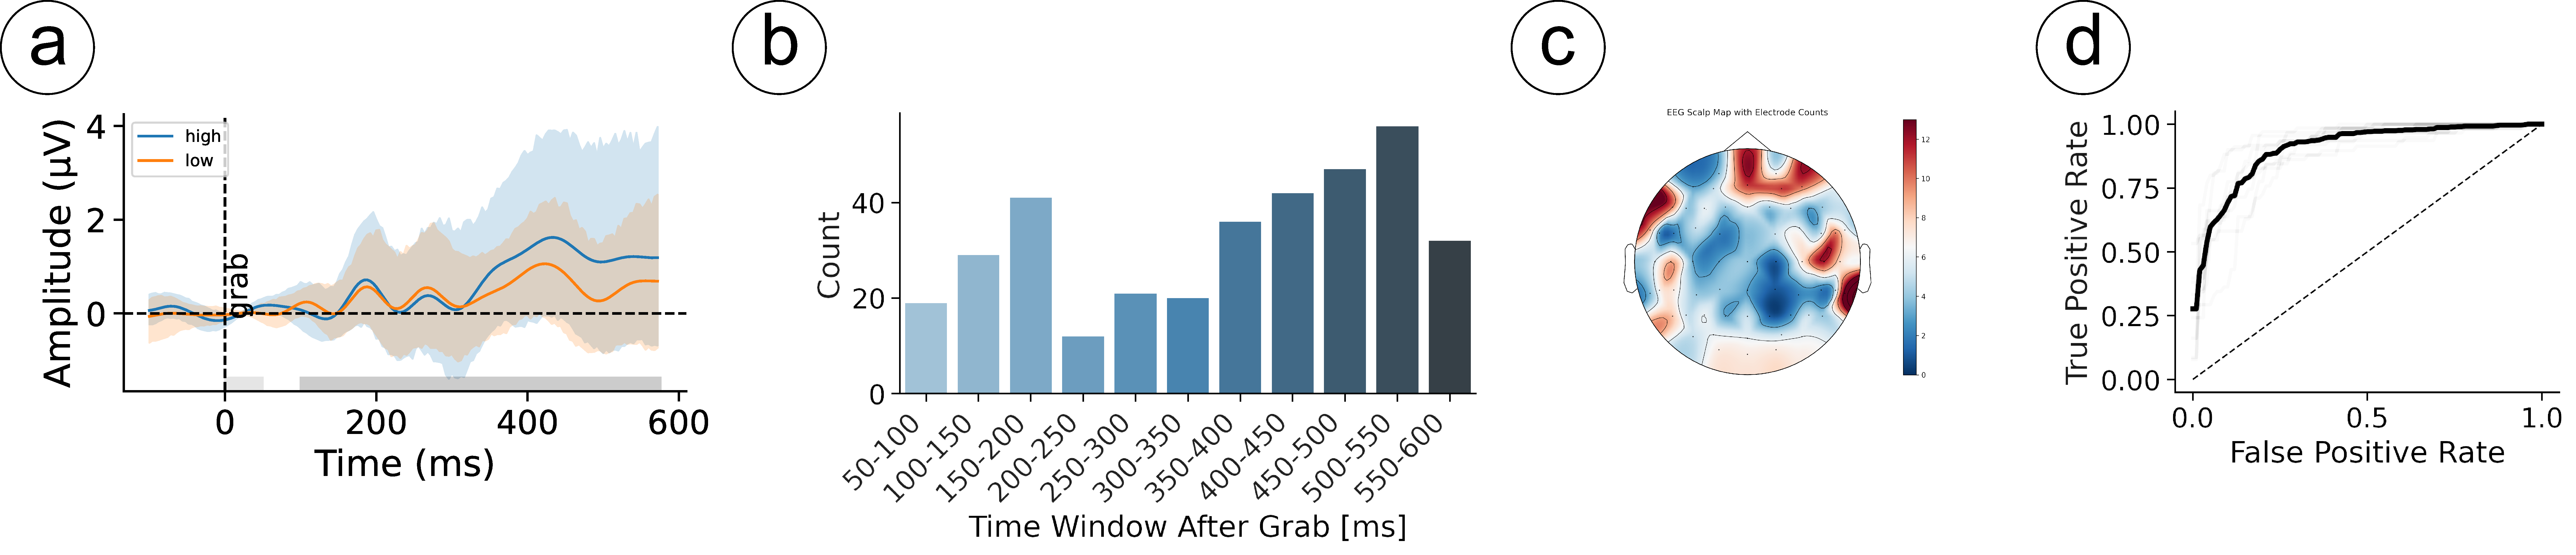
\includegraphics[width=\linewidth]{input/img/eeg_results.pdf}
    \caption{\textit{a:} ERP at CZ for the preference split; \textit{b:} number of times time window was selected for classification; \textit{c:} number of times channel was selected for classification; \textit{d:} ROC curves for all participants. The dashed diagonal line represents random classification, while the solid curves indicate model performance.}
    \Description{Receiver Operating Characteristic (ROC) curves for all participants. The True Positive Rate (sensitivity) is plotted against the False Positive Rate at varying decision thresholds. The dashed diagonal line represents the performance of a random classifier (i.e., no discrimination ability). The solid curves indicate that the models exhibit strong discriminative power, as they are positioned well above the diagonal reference line.}
    \label{res:roc}
\end{figure*}